\chapter{Reference Implementations}
\label{reference}

%%%%%%%%%%%%%%%%%%%%%%%%%%%%%%%%%%%%%%%%%%%%%%%%%%%%%%%%%%%%%%%%%%%%%%%%%%%%%%%%%%%%%%%%%%%

\section{Verilog reference implementations}

We have implemented Verilog coers for all instructions proposed in this
specification. These cores are permissively licensed under the ISC license and
can be obtained from \url{https://github.com/riscv/riscv-bitmanip/tree/master/verilog}.

\begin{figure}[t]
\begin{center}
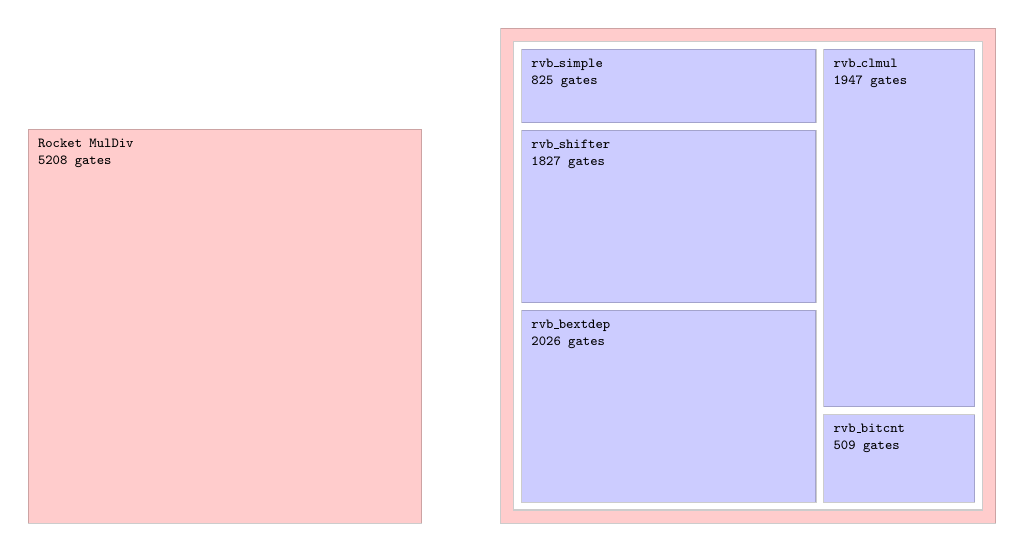
\begin{tikzpicture}
\draw [fill=red, opacity=0.2] (-6.000000,0) rectangle (-1,5.000000);
\node (label) at (-6.000000,5.000000) [below right, align=left, style={font=\tiny\tt}] {Rocket MulDiv \\ 5208 gates};
\draw [fill=red, opacity=0.2] (0,0) rectangle (6.285422,6.285422);
\draw [draw=black!20, fill=white] (0.166733,0.166733) rectangle (6.118689,6.118689);
\draw [draw=black, fill=blue, opacity=0.2] (0.266733,0.266733) rectangle (4.004054,2.701163);
\node (label) at (0.266733,2.701163) [below right, align=left, style={font=\tiny\tt}] {rvb\_bextdep \\ 2026 gates};
\draw [draw=black, fill=blue, opacity=0.2] (0.266733,2.801163) rectangle (4.004054,4.986653);
\node (label) at (0.266733,4.986653) [below right, align=left, style={font=\tiny\tt}] {rvb\_shifter \\ 1827 gates};
\draw [draw=black, fill=blue, opacity=0.2] (0.266733,5.086653) rectangle (4.004054,6.018689);
\node (label) at (0.266733,6.018689) [below right, align=left, style={font=\tiny\tt}] {rvb\_simple \\ 825 gates};
\draw [draw=black, fill=blue, opacity=0.2] (4.104054,0.266733) rectangle (6.018689,1.379536);
\node (label) at (4.104054,1.379536) [below right, align=left, style={font=\tiny\tt}] {rvb\_bitcnt \\ 509 gates};
\draw [draw=black, fill=blue, opacity=0.2] (4.104054,1.479536) rectangle (6.018689,6.018689);
\node (label) at (4.104054,6.018689) [below right, align=left, style={font=\tiny\tt}] {rvb\_clmul \\ 1947 gates};
\end{tikzpicture}
\end{center}
\caption{Area of 32-bit Rocket MulDiv core (left) compared with a complete implementation of all 32-bit instructions
proposed in this specification except CRC instructions (right).}
\label{refhw32}
\end{figure}

For evaluation purposes we synthesized these cores for RV32 and RV64 to the following mockup ASIC cell library:

\begin{center}
\begin{tabular}{ll}
Cell & Cate Count \\
\hline
NOT   & 0.5 \\
NAND  & 1   \\
NOR   & 1   \\
XOR   & 3   \\
XNOR  & 3   \\
DFF   & 4   \\
\end{tabular}
\hfil
\begin{tabular}{ll}
Cell & Cate Count \\
\hline
AOI3  & 1.5 \\
OAI3  & 1.5 \\
AOI4  & 2   \\
OAI4  & 2   \\
NMUX  & 2.5 \\
MUX   & 3 \\
\end{tabular}
\end{center}

For comparison we also synthesized the rocket-chip MulDiv cores obtained using the following
rocket-chip configurations:

\begin{verbatim}
  class MulDivConfig64 extends Config(
      new WithFastMulDiv ++
      new DefaultConfig
  )

  class MulDivConfig32 extends Config(
      new WithRV32 ++
      new WithFastMulDiv ++
      new DefaultConfig
  )
\end{verbatim}

The following table lists the verilog reference cores and the instructions they implement:

\begin{center}
\begin{tabular}{lp{6cm}}
Module & Instructions \\
\hline
\tt rvb\_bextdep  & bext bdep grev gorc shfl unshfl                                               \\
\tt rvb\_clmul    & clmul clmulr clmulh                                                           \\
\tt rvb\_shifter  & sll srl sra slo sro rol ror fsl fsr slliu.w sbset sbclr sbinv sbext bfp       \\
\tt rvb\_bmatxor  & bmatxor bmator                                                                \\
\tt rvb\_simple   & min max minu maxu andn orn xnor pack cmix cmov addiwu addwu subwu adduw subuw \\
\tt rvb\_bitcnt   & clz ctz pcnt bmatflip                                                         \\
\tt rvb\_full     & All of the above                                                              \\
\end{tabular}
\end{center}

On RV64 these cores also implement all {\tt *W} instruction variants of the above instructions.

Note that {\tt rvb\_shifter} also implements the base ISA {\tt sll}, {\tt srl},
and {\tt sra} instructions. Thus it can replace an existing implementation of
the base ISA shift instructions.

Fig.~\ref{refhw32} shows the area comparison for RV32 and fig.~\ref{refhw64} shows the comparison for RV64.
The area of the red frame surrounding the blue {\tt rvb\_*} modules accurately represents the added area
by the {\tt rvb\_full} wrapper module.

\begin{figure}[t]
\begin{center}
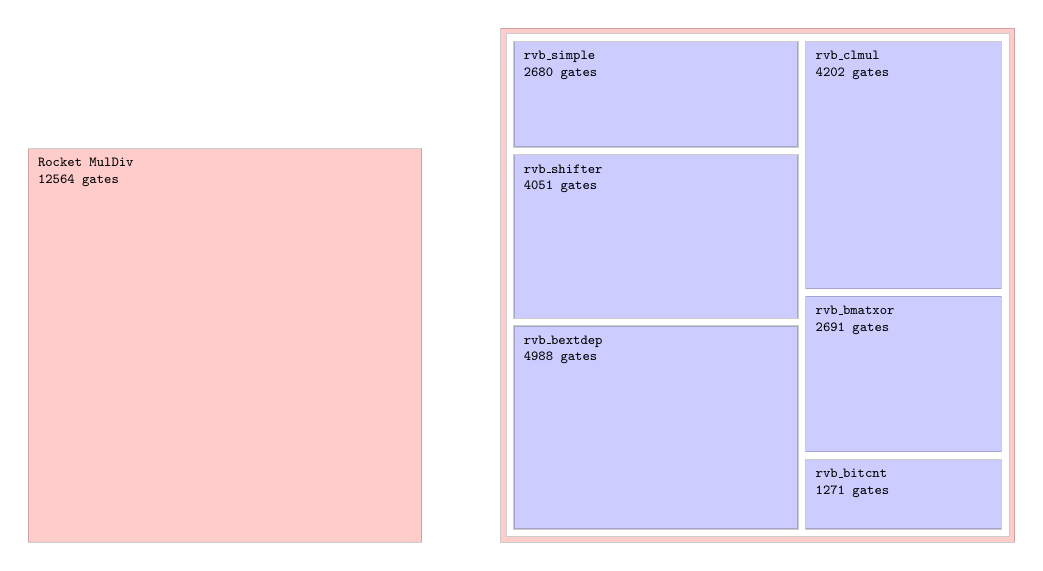
\begin{tikzpicture}
\draw [fill=red, opacity=0.2] (-6.000000,0) rectangle (-1,5.000000);
\node (label) at (-6.000000,5.000000) [below right, align=left, style={font=\tiny\tt}] {Rocket MulDiv \\ 12564 gates};
\draw [fill=red, opacity=0.2] (0,0) rectangle (6.528688,6.528688);
\draw [draw=black!20, fill=white] (0.069370,0.069370) rectangle (6.459318,6.459318);
\draw [draw=black, fill=blue, opacity=0.2] (0.169370,0.169370) rectangle (3.776653,2.746583);
\node (label) at (0.169370,2.746583) [below right, align=left, style={font=\tiny\tt}] {rvb\_bextdep \\ 4988 gates};
\draw [draw=black, fill=blue, opacity=0.2] (0.169370,2.846583) rectangle (3.776653,4.920879);
\node (label) at (0.169370,4.920879) [below right, align=left, style={font=\tiny\tt}] {rvb\_shifter \\ 4051 gates};
\draw [draw=black, fill=blue, opacity=0.2] (0.169370,5.020879) rectangle (3.776653,6.359318);
\node (label) at (0.169370,6.359318) [below right, align=left, style={font=\tiny\tt}] {rvb\_simple \\ 2680 gates};
\draw [draw=black, fill=blue, opacity=0.2] (3.876653,0.169370) rectangle (6.359318,1.048611);
\node (label) at (3.876653,1.048611) [below right, align=left, style={font=\tiny\tt}] {rvb\_bitcnt \\ 1271 gates};
\draw [draw=black, fill=blue, opacity=0.2] (3.876653,1.148611) rectangle (6.359318,3.121890);
\node (label) at (3.876653,3.121890) [below right, align=left, style={font=\tiny\tt}] {rvb\_bmatxor \\ 2691 gates};
\draw [draw=black, fill=blue, opacity=0.2] (3.876653,3.221890) rectangle (6.359318,6.359318);
\node (label) at (3.876653,6.359318) [below right, align=left, style={font=\tiny\tt}] {rvb\_clmul \\ 4202 gates};
\end{tikzpicture}
\end{center}
\caption{Area of 64-bit Rocket MulDiv core (left) compared with a complete implementation of all 64-bit instructions
proposed in this specification except CRC instructions (right).}
\label{refhw64}
\end{figure}

Regarding timing we evaluate the longest paths for {\tt rvb\_full} and
rocket-chip {\tt MulDiv}, measured in gate delays:

\begin{center}
\begin{tabular}{lcc}
& RV32 & RV64 \\
\hline
\tt rvb\_full & 30 & 57 \\
\tt MulDiv & 43 & 68 \\
\end{tabular}
\end{center}

All {\tt rvb\_*} reference cores provide single-cycle implementations of their functions,
with the exception of {\tt rvb\_clmul} which requires 4 cycles for a 32-bit
carry-less multiply and 8 cycles for a 64-bit carry-less multiply.

%%%%%%%%%%%%%%%%%%%%%%%%%%%%%%%%%%%%%%%%%%%%%%%%%%%%%%%%%%%%%%%%%%%%%%%%%%%%%%%%%%%%%%%%%%%

\section{Fast C reference implementations}
\label{fastc}

GCC has intrinsics for the bit counting instructions {\tt clz}, {\tt ctz}, and
{\tt pcnt}.  So a performance-sensitive application (such as an emulator)
should probably just use those:

\input{bextcref-fast-bitcnt}

For processors with BMI2 support GCC has intrinsics for bit extract and bit
deposit instructions (compile with {\tt -mbmi2} and include {\tt <x86intrin.h>}):

\input{bextcref-fast-bext-bmi2}

For other processors we need to provide our own implementations. The following
implementation is a good compromise between code complexity and runtime:

\input{bextcref-fast-bext}

For the other Bitmanip instructions the C reference functions given in Chapter~\ref{bext}
are already reasonably efficient.
